\documentclass[a4paper]{article}
\usepackage{amsmath}
\usepackage{amssymb}
\usepackage{fancyhdr}
\usepackage{a4wide}
\usepackage{geometry}
\usepackage[utf8]{inputenc}
\usepackage{graphicx}
\geometry{a4paper,left=2cm,right=2cm, top=3cm, bottom=3cm}
\usepackage{listings}
\lstset{language=xml}
\newcommand{\oh}[1]{$\mathcal{O}(#1)$}
\newcommand{\titel}[1]{\fancyhead[C]{#1}}
\newcommand{\name}{\fancyhead[L]{Alexander Landmesser}}
\newcommand{\matrikel}{\fancyhead[R]{}}
\newcommand{\pl}{\hspace*{1cm}}
\begin{document}
\title{Ausgewählte Kapitel ADS}
\maketitle
\section{Datenstrukturen für Mengen}
\subsection{Union-Find-Problem}
Verwaltung von diskunkten Mengen\\
%TODO BILD 1: Mengen Beispiel
\subsubsection*{Problem}
Verwalte eine Partition (Zerlegung in disjunkte Teilmengen) der Menge \{1,...,n\} unter folgenden Operationen.\\
Jede Teilmenge (Block) besitzt einen eindeutigen Namen aus \{1,..,n\}.
\begin{itemize}
\item FIND(x): $x\in \{1,..,n\}$ Liefert den Namen der Teilmenge, die x enthält
\item UNION(A,B,C): Vereinigt die Teilmengen mit Namen A und B zu einer Teilmenge mit dem Namen C.
\end{itemize}
\subsubsection*{Initialisierung}
Wir starten mit der Partitionierung: $\{\{1\},..,\{n\}\}$ mit dem Namen $i$ für $\{i\}$,$1\leq i \leq n$\\
Analyse: Kosten für 1 Union (worst case)\\
Amortisiert: Kosten für $n-1$ mögliche UNIONs\\
$\rightarrow$ Kosten von $n-1$ UNIONs und m FINDs\\
\subsubsection*{Lösungen}
\underline{\textbf{1. Lösung} (einfach)}\\
Verwende ein Feld name[1..n] mit name[x] = Name des Blocks der x enthält. $1\leq x \leq n$\\
\begin{lstlisting}
for i=1 to n do
	name[i] <- i
od
\end{lstlisting}
FIND(x): return name[x] : \oh{n}\\
UNION(A,B,C): \oh{n}
\begin{lstlisting}
for i=1 to n do
	if name[i] = A OR name[i] = B
	then name[i] <- C
	fi
od
\end{lstlisting}
Gesamtlaufzeit (Lemma 1):\\
$n-1$ UNIONs und m FINDs kosten \oh{n^2+m}\\
\underline{\textbf{2. Lösung} (Verbesserung)}\\
1. Find unverändert\\
2. Ändere den Namen der kleineren Menge in den Namen der größeren (Relabel the smaller half)\\
Zusätzliche Felder:
\begin{itemize}
\item size[1..n]: size[A] = Anzahl Elemente im Block A, initialisiert mit 1
\item L[1..n]: L[A] = Liste aller Elemente in Block A, initialisiert L[i] = \{i\}
\end{itemize}
FIND(x) bleibt gleich\\
UNION(A,B):
\begin{lstlisting}[escapechar=!]
if size[A] !$\leq$! size[B]
then
	forall i in L[A] do
		name[i]!$\leftarrow$! B
	od
	size[B] += size[A]
	L[B] !$\leftarrow$! L[B] concatenate L[C]
else
	symmetrisch
\end{lstlisting}
Die Menge heißt jetzt A oder B\\
Effekt: UNION(A,B,..) hat Laufzeit \oh{min(|A|,|B|)}\\
Worst Case eines UNION dieser Folge von UNIONs: \oh{\frac{n}{2}} = \oh{n} (kann nur einmal vorkommen)\\
Wie oft kann sich name[x] für ein bestimmtes $x:1\leq x\leq n$ ändern?\\
Beobachtung:
\begin{itemize}
\item Am Anfang ist jedes Element x in einer ein-elementigen Menge
\item Am Ende sind alle Elemente in einer Menge der Größe n
\item Immer wenn ein Element x seinen Namen ändert befindet es sich danach in einer doppelt so großen Menge (nach dem UNION)
\end{itemize}
$\Rightarrow$ Jedes Element $x\in \{1,..,\}$ kann maximal $log(n)$ mal seinen Namen ändern.\\
\underline{Satz 1:}
Bei UNION-FIND mit "Relabel the smaller half" sind die Gesamtkosten einer beliebigen Folge von n-1 UNIONS und m Finds \oh{m+n*log(n)}\\
Im Schnitt (amortisiert) kostet ein UNION $log(n)$\\
\underline{\textbf{3. Lösung}}\\
Lösung 1 und 2 haben FIND effizient gelöst, hier UNION\\
Jeder Block wird als Baum dargestellt. Die Knoten repräsentieren die Elemente des Blocks. In der Wurzel steht der Name des Blocks.\\
%TODO BILD 2: Bäume der Mengen
UNION(A,B,E): Mache die Wurzel von A zum Kind der Wurzel von B und nenne die Wurzel um in E.\\
FIND(x): Starte bei Element (Knoten) x und laufe bis zur Wurzel, dort steht der Name $\rightarrow$ \oh{Tiefe\ von\ x}\\
\textbf{Realisierung der Datenstruktur durch Felder:}\\
$vater[i]=\left\lbrace \begin{array}{c}Vater\ von\ i\ in\ seinem\ Baum\\ 0,\ falls\ i\ Wurzel\end{array}\right.$\\ %HELP
$name[i]=$Name des Blocks mit Wurzel i (at nur Bedeutung, falls i Wurzel)\\
$wurzel[i]=$ Wurzel des Blocks mit Namen i\\
\begin{tabular}{ l c r }
Initialisierung: & FIND(x): & UNION(A,B,C):\\
\begin{lstlisting}
for i=1 to n do
	vater[i] = 0
	name[i] = i
	wurzel[i] = i
od
\end{lstlisting}
&
\begin{lstlisting}
while vater[x] != 0 do
	x = vater[x]
od
return name[x]
\end{lstlisting}&
\begin{lstlisting}
r1 = wurzel[A]
r2 = wurzel[B]
vater[r1] = r2
name[r2] = C
wurzel[C] = r2
\end{lstlisting}

\end{tabular}\\
Analyse:
\begin{itemize}
\item UNION: \oh{1} worst case
\item FIND(x): Tiefe von x (max Höhe des entstehenden Baums, n-1 möglich)
\end{itemize}
\underline{\textbf{4. Lösung (Weighted Union rule):}}\\
Vermeide große Tiefen, dafür hänge den kleineren Baum (Anzahl Knoten) an den größeren\\
Alternativ: Hänge den Baum mit kleinerer höhe an den tieferen.\\
Realisierung: Zusätzliches Feld\\
size[i] = Anzahl Knoten um Unterbaum mit Wurzel i\\
\begin{tabular}{ l c r }
Initialisierung: & FIND(x) (wie bei 3): & UNION(A,B,C):\\
\begin{lstlisting}
for i=1 to n do
	vater[i] = 0
	name[i] = i
	wurzel[i] = i
	size[i] = 1
od
\end{lstlisting}
&
\begin{lstlisting}[escapechar=|]
while vater[x] != 0 do
	x = vater[x]
od
return name[x]
\end{lstlisting}&
\begin{lstlisting}
r1 = wurzel[A]
r2 = wurzel[B]
if size[r1] |$\leq $| size[r2] then
	vater[r1] = r2
	name[r2] = C
	wurzel[C] = r2
	size[r2] += size[r1]
else
	symmetrisch
\end{lstlisting}
\end{tabular}
Zeige Laufzeit \oh{log(n)}:\\
Sei für jeden Knoten x die höhe(x) die Hohe von x in seinem Baum (maximale Pfad zu Blatt), Blatt=0\\
size(x): Anzahl der Knoten im Unterbaum mit Wurzel x (Gewicht)\\
\underline{Lemma}: Bei weighted Union rule gilt stets, dass $size(x)\geq 2^{\text{höhe}(x)}$ für alle Knoten x.\\
Beweis: Induktion über höhe(x):\\
\begin{lstlisting}[escapechar=!]
Vorasussetzung:
	h!ö!he(x) = 0: x ist Blatt -> size(x)=1=!$2^0$!
Anfang:
	size(y) !$\geq 2^{\text{höhe}(y)}$!
Schritt:
	Sei h!ö!he(x) > 0
	Sei y ein Kind von x mit h!ö!he(x)-1
	Betrachte die UNION Operation bei der x zum Vater von y wurde.
	Seien !$\overline{size}(x)$! und !$\overline{size}(y)$! die Gewichte vor der UNION Operaion, dann gilt:
	1) size(y) = !$\overline{size}(y)$!, da sich das Gewicht nur !für! Wurzeln !ä!ndern kann
	2) !$\overline{size}(x) \geq \overline{size}(y)$! durch weighted union rule
	3) Nach der Operation: !$size(x) \geq \overline{size}(x)+\overline{size}(y)$!
		!$\geq 2*\overline{size}(y)$! wegen 2.
		!$\geq 2*size(y)$! wegen 1.
		!$\geq 2*2^{\text{höhe}(y)}$! nach IA
		!$=2^{\text{höhe}(y)+1} = 2^{\text{höhe}(x)}$!
\end{lstlisting}
Da Anzahl der Knoten $n \Rightarrow size(x) \leq n$ gilt:\\
\hspace*{1cm}$\Rightarrow n\geq size(x)\geq 2^{hoehe(x)}$ für alle x\\
\hspace*{1cm}$hoehe(x) \leq log(n)$\\
\underline{Satz:} Bei UNION-FIND mit weighted UNION ist die Laufzeit einer beliebigen Folge n-1 Unions und m Finds \oh{n+log(n)}\\
Beweis: 1. UNION \oh{1} worst-case, 2. Find \oh{log(n)} worst case (Lemma)\\
\underline{\textbf{5. Lösung (Verbesserung von FIND):}}\\
Pfad-Komprimierung (path compression)\\
Ein FIND(x) durchläuft den Pfad von x zur Wurzel.\\
$x=x_0,...,x_l=Wurzel$\\
\underline{Idee:} Hänge $x_0,...,x_{l-1}$ direkt an die Wurzel an.\\
Erhöht die Kosten dieses Finds um einen konstanten Faktor.\\
Algorithmus:
\begin{lstlisting}
FIND(x)
	r <- x;
	while vater[r] != 0 do 
		r <- Vater[r]
	od
	while x != r do
		y <- vater[x]
		vater[x] <- r
		x <= y
	od	
\end{lstlisting}
Ganz klar: \oh{log(n)} worst case\\
\underline{Satz (Tarjan):} Bei UNION-FIND mit weighted UNION und path compression hat eine beliebige Folge von n-1 Unions und m Finds mit $m\geq n$, die Gesamtkosten \oh{m*\alpha(m,n)}, \\wobei $\alpha(m,n) = min\lbrace z\in \mathbb{N} | A(z,\frac{4m}{n}) > log n\rbrace$\\
mit A einer Variante der Ackermannfunktion.\\
$\alpha$ ist eine Art Inverse der Ackermannfunktion $\Rightarrow$ Ist extrem langsam wachsend.\\
Definition von A:\\
$A: \mathbb{N}_0\times\mathbb{N}_0 \rightarrow \mathbb{N}_0$\\
$A(i,0) = 0$ für alle $i\in\mathbb{N}_0$\\
$A(0,x) = 2x$ für alle $x\geq 1$\\
$A(i,1) = 2$\\
$A(i,x) = A(i-1,A(i,x-1))$ für $i\geq 1,x\geq 2$\\
A(i,x) als Matrix $i\times x$: 
$\begin{matrix}
0&2&4&6&8&10\\
0&2&4&8&16&32\\
0&2&4&16&65536&2^{65536}&\\
0&2&4&65536&2\uparrow\uparrow65536&.\\
0&2&.&.&.&.
\end{matrix}
$\\
1. Zeile: $A(0,x)=2x$; 2. Zeile: $A(1,x)=2^x$; 3. Zeile: $A(2,x)=2^{2^{.^{.^2}}}$\\
Anmerkung: Pfeilschreibweise=(Knuth Up-Arrow)\\
Beweis des Satzes:\\
Situation: n Elemente \{1,..,n\}, beliebige Folge von n-1 Unions und m Finds: $U_1,F_1,F_2,U_2,...$\\
Am Ende: 1 Baum T' (n-1 weighted Unions)\\
Konzeptuell kann T' anders erhalten werden: Führe zunächst alle Unions aus $\rightarrow$ Baum T. Dann führe m partielle Finds auf T aus ($PF_1,...,PF_m$), die genau den selben Pfad wir $F_i$ durchlaufen, bis zu ihrere ursprünglichen Wurzel vor den Unions.\\
Wir schätzen nun die Gesamtkosten dieser Folge (insbesondere der m PF's) ab.\\
Frage: Wieviele Vater-Verweise (Kanten) werden insgesamt durchlaufen?\\
Sei F=Multi-Menge aller durch die PF's durchlaufenen Kanten (mit Mehrfachen)\\
Zu zeigen: $|F| = $\oh{m*\alpha(m,n)}\\
Idee:\\
a) Teile F in Gruppen nach Rang der Endpunkte der Kanten, wobei Rang(x)=Höhe(x) im Baum T (nicht T')\\
b) Schätze die Gruppen einzeln ab.\\
Zunächst einteilung der Knoten in die Gruppen nach Rang (nicht disjunkt).\\
Sei $z\in\mathbb{N}_0$, Für $0\leq i \leq z, j\geq 0$ sei:\\
$G_{ij}=\lbrace Knoten\ x|A(i,j)\leq Rang(x)<A(i,j+1)\rbrace$\\
Veranschaulichung: $\lbrace [A(i,j) ... A(i,j+1)[\rbrace$ Menge von Ineraktionen\\
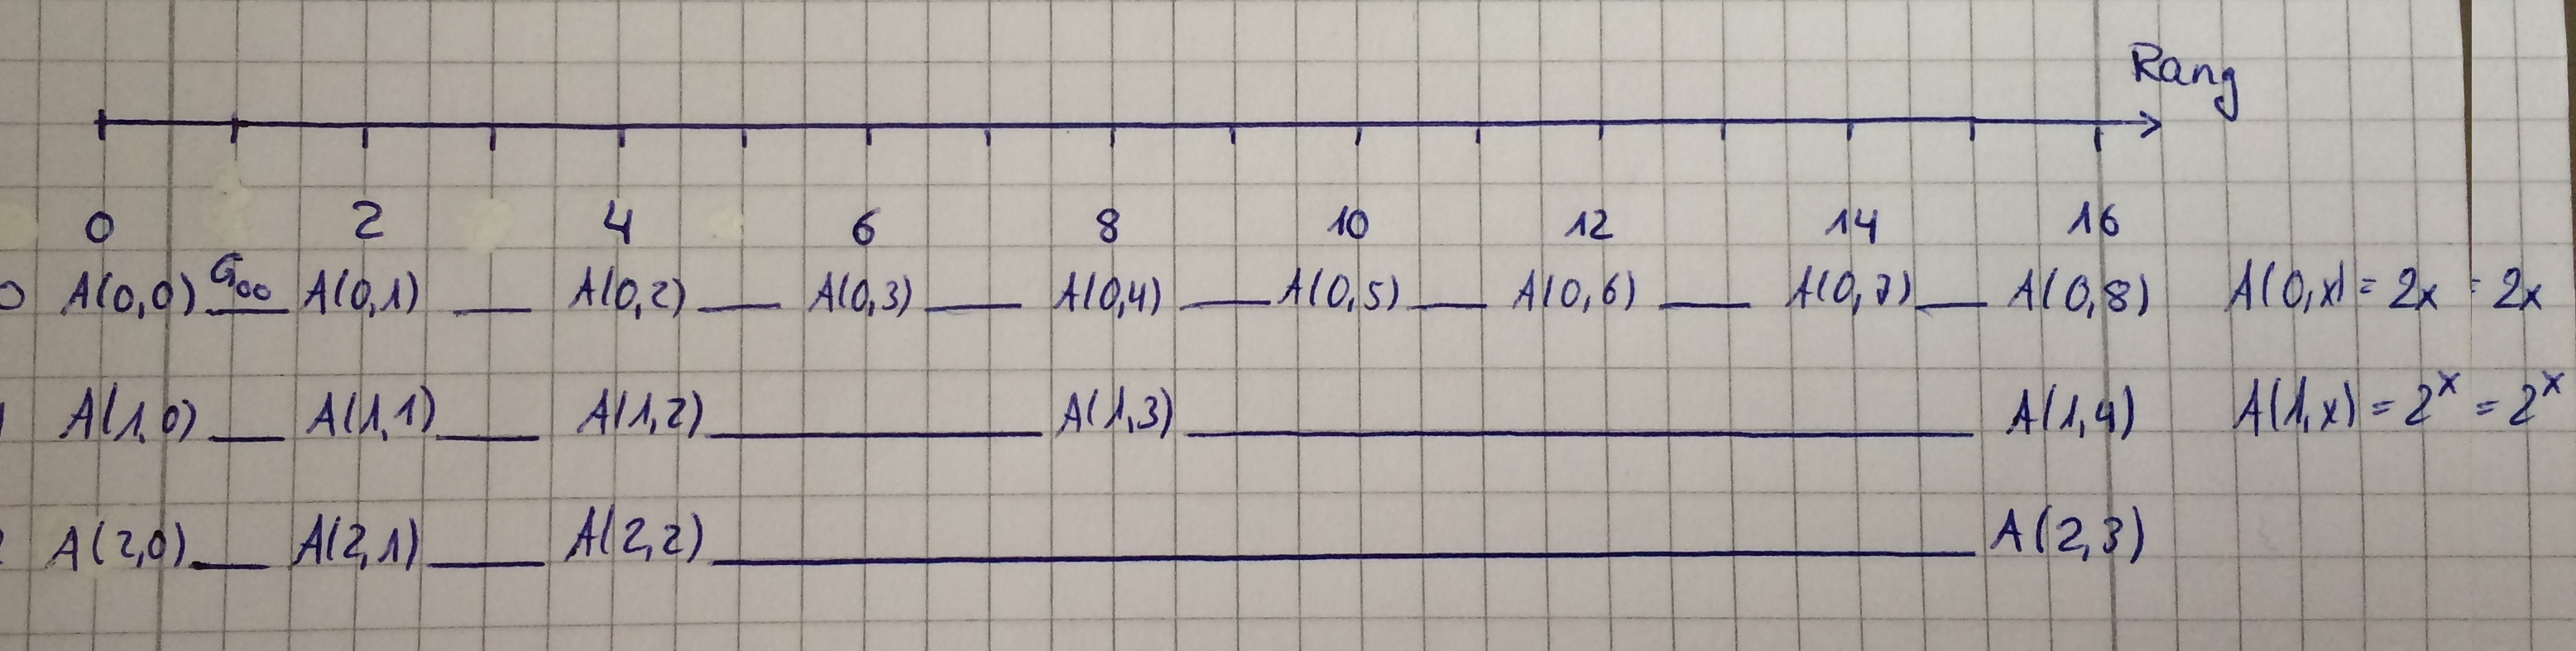
\includegraphics[scale=0.15]{Bild3.png}\\
Beispiel: Rang(x)=7, Rang(y)=13\\
$\Rightarrow$ $x\in G_{0,3},G_{1,2},G_{2,2},...$\\
$\Rightarrow$ $y\in G_{0,6},G_{1,3},G_{2,2},...$\\
Eine Einteilung der Multi-Menge F \\
Für $0\leq k \leq z: N_k=\lbrace (x,y)\in F | k=min\lbrace i\geq 0|\exists j\ mit\ x,y\in G_{i,j}\rbrace\rbrace$\\
und $N_{z+1} := F\setminus\cup_{0\leq i\leq z} N_i$\\
Schließlich definieren wir für $0\leq k\leq z+1: L_k=\lbrace(x,y)\in N_k | (x,y) $ist letzte (oberste) Kante auf PF-Pfad\\
\underline{Lemma:}\\
a) $|L_k| \leq m$ für $0\leq k \leq z+1$\\
b) $|N_0\setminus L_0|\leq n$\\
c) $|N_k\setminus L_k | \leq \frac{5}{8}n$ für $1\leq k \leq z$\\
d) $|N_{z+1}\setminus L_{z+1} | \leq n*a(z,n)$ mit $a(z,n) = min\lbrace i\geq 0 | A(z,i) > log(n)\rbrace$\\
Beweis:\\
a) Für jedes PF gibt es höchstens 1 Kante in $L_k$. Die Behauptung folgt daraus, dass es insgesamt nur m PFs gibt.\\
b) Sei $(x,y)\in N_0\setminus L_0$, dann gilt $\exists j\geq 0$ mit $x,y \in G_{0,j}$, das heißt $A(0,j) \leq Rang(x) < Rang(y) < A(0,j+1)$\\
\hspace*{1cm}$\Rightarrow Rang(x)=2j, Rang(y)=2j+1$\\
\hspace*{1cm}$(x,y) \not\in L_0 \Rightarrow $ nicht die letzte Kante in diesem PF: Betrachte PF von (x,y), dann existiert eine Kante $(s,t)\in L_0$ auf diesem PF-Pfad\\
Situation:\\
$Rang(x)=2j, Rang(y)=2j+1$\\
$Rang(s)\geq Rang(y)$ da letzter Pfad vor dem nicht letzten sein muss\\
$Rang(t) > Rang(s)$ da Pfad von s nach t\\
$\Rightarrow Rang(t) \geq 2j+2$\\
Nach dem PF: x hat neuen Vater (möglicherweise t) u mit $Rang(u)\geq Rang(t)\geq 2k+2$\\
$\Rightarrow$ Rangdifferenz zwischen x und dem neuen Vater u $\geq 2$\\
$\Rightarrow$ Spätere PFs können keine Kante (x,..) mehr zu $N_0$ hinzufügen\\
$\Rightarrow$ Für jeden Knoten wird maximal eine ausgehende Kante (Vaterverweis) in $N_0\setminus L_0$ gezählt werden.\\
$\Rightarrow |N_0\setminus L_0| \leq n$\\
Beweis c), d):\\
Idee: Schätze Beitrag eines Knotens $x\in G_{k,j}$ zu $N_k\setminus L_k$ d.h. alle Kanten, die von x ausgehen und in $N_k\setminus L_k$ gezählt werden.\\
Sei $k\geq 1$ und $x\in G_{k,j}$ beliebig, d.h. $\exists j$ mit $ A(k,j) \leq Rang(x) < A(k,j+1)$\\
und $y_1,...,y_q$ alle Endknoten mit $(x,y_i)\in N_k\setminus L_k$. Ziel: q nach oben abschätzen.\\
$\Rightarrow Rang(y_1)\leq ...\leq Rang(y_q)<A(k,j+1)$\\
Beobachtungen:\\
1) $j\geq 2$ weil sonst k=0 die minimale Zeile definiert, sodass $(x,y_i)$ im selben Intervall ( de ersten 3 Spalten sind immer gleich gefüllt mit 0,2,4). Hier: $k\geq 1$\\
2) $(x,y_i)\not\in L_k$ für $1\leq i\leq q \Rightarrow \exists (s_i,t_i)\in N_k$ auf PF-Pfad von $(x,y_i)$ oberhalb von $(x,y_i)$
\end{document}